\begin{frame}
	\frametitle{Implémentation}	
	
	Côté serveur :
	\begin{itemize}
		\item Java
		\item un thread d'émission (broadcast)
		\item un thread de réception par client connecté
	\end{itemize}

	Côté client :
	\begin{itemize}
		\item Java
		\item un thread d'émission
		\item un thread de réception
	\end{itemize}

\end{frame}

\begin{frame}
	\frametitle{Gestion des évènements}
	\begin{figure}
		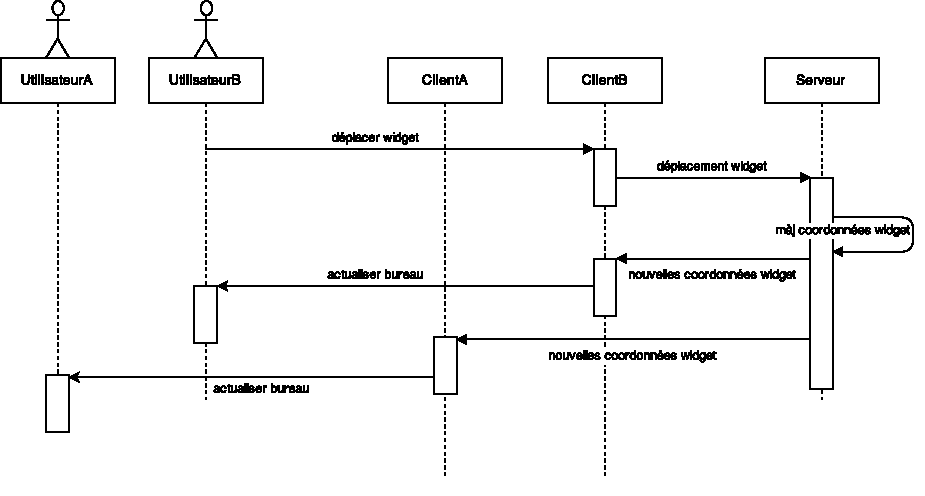
\includegraphics[scale=0.7]{resources/DI2.pdf}
		\caption{Gestion des mises à jour du bureau}
	\end{figure}
\end{frame}

\begin{frame}
	\frametitle{IHM}
	\begin{itemize}
		\item Utilisation de Swing
		\item Rafraîchissement de la vue dès mise à jour bureau
	\end{itemize}
\end{frame}